\section{Conception}
\noindent
Dans cette partie, nous allons présenter le diagramme de séquence correspondant à notre diagramme cas d'utilisation précédemment présentés dans les descriptions textuelles pour le deuxième Sprint.

\subsection{Diagramme de séquence détaillé}
\noindent
Nous avons regroupé les deux cas d'utilisation << Rechercher produits en Arabe traditionnel >> et << Rechercher produits en Arabe en dialecte Tunisien >> dans un seul diagramme de séquence présenté dans la figure ~\ref{fig:diagseqsprint2}.

\begin{figure}[H]
	\centering
	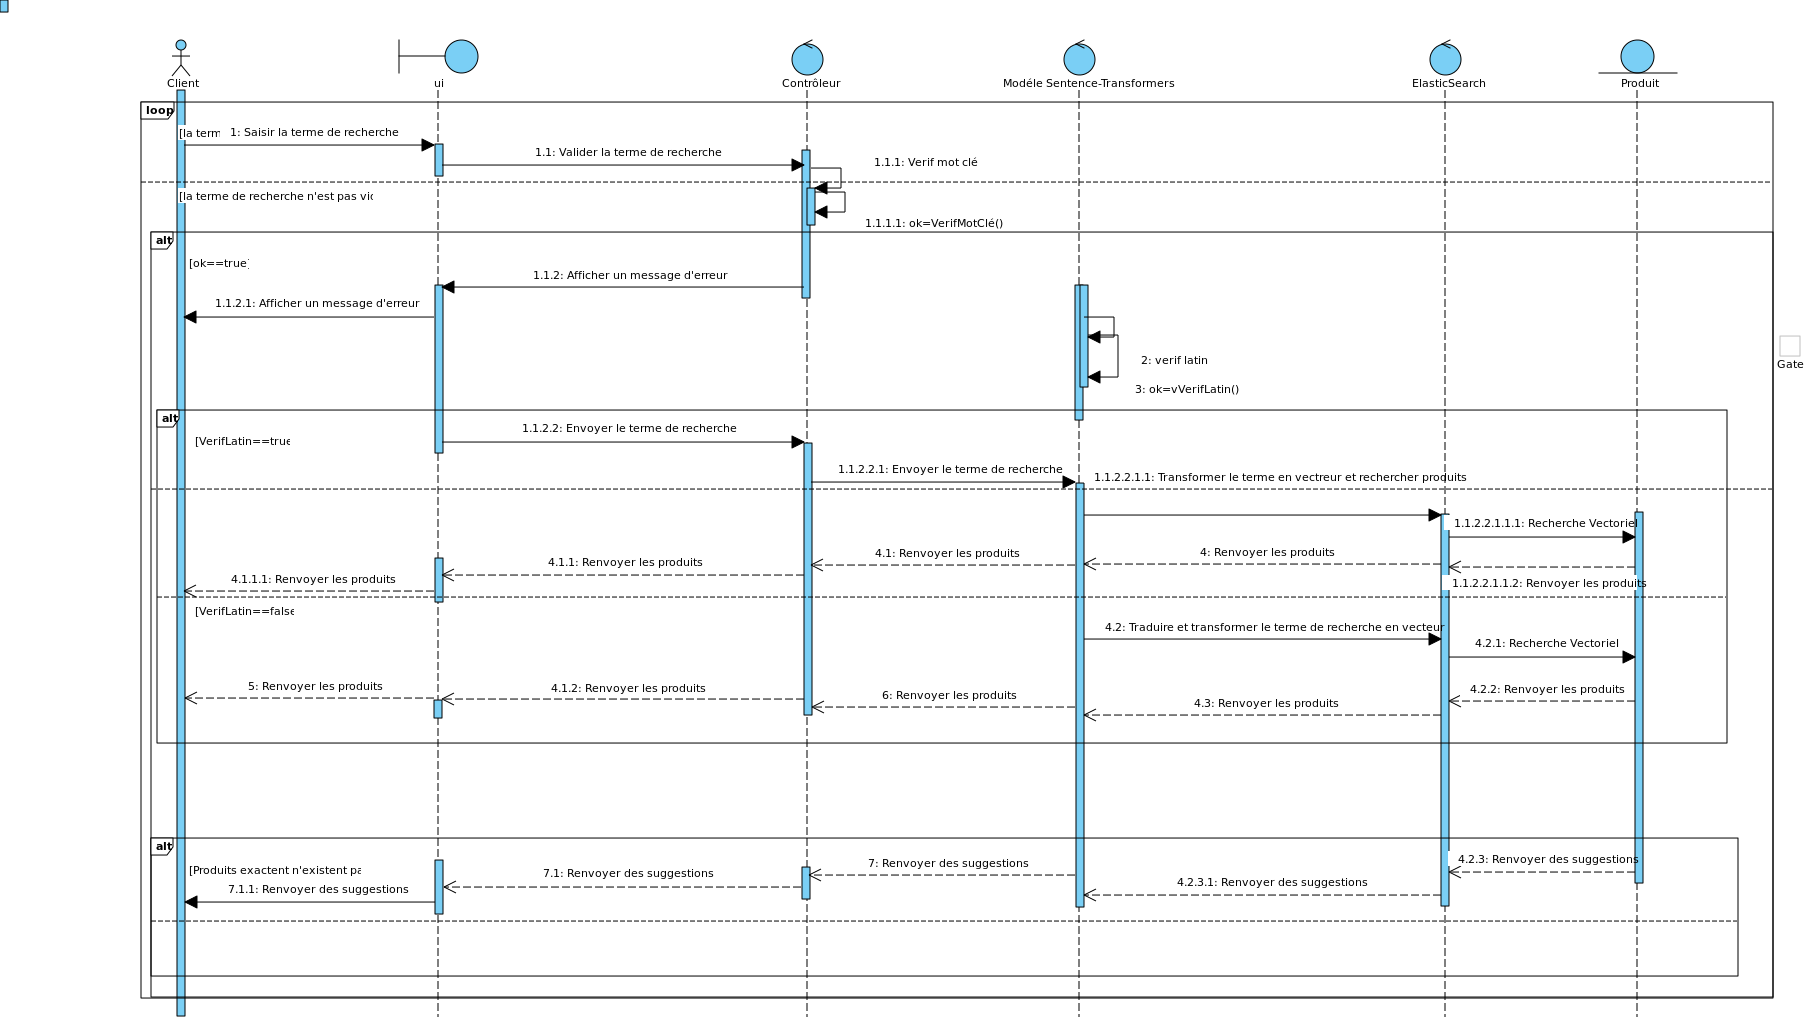
\includegraphics[width=1\textwidth]{logos/seqsprint2.png}
	\caption{Diagramme de séquence des cas d’utilisations « Rechercher produits en Arabe Traditionnel » et << Rechercher produits en Arabe en dialecte Tunisien >>}
	\label{fig:diagseqsprint2}
\end{figure}

\section{Réalisation}
\noindent
Cette partie est consacrée à la présentation des étapes nécessaires pour réaliser le travail nécessaire pour satisfaire notres cas d'utilisations, qui consiste à permettre le client ou le visiteur à rechercher notres produits en Arabe traditionnel et Arabe en dialecte tunisien tout en améliorant l'expérience de recherche en utilisant la traduction et la recherche vectorielle via Elasticsearch.

\newpage
\subsection{Les premières approches}
\noindent